\documentclass{article}
\usepackage[utf8]{inputenc}

\title{CSE 4701 — Project 1, Part 1}
\author{Mike Medved}
\date{September 26th, 2023}

\usepackage{graphicx}
\usepackage{amsthm}
\usepackage{amssymb} 
\usepackage{amsmath}
\usepackage{caption}
\usepackage{listings}
\usepackage{multirow, tabularx}
\usepackage[margin=1in]{geometry} 
\usepackage[table,xcdraw]{xcolor}
\usepackage{enumitem}
\newlist{parlist}{enumerate}{1}
\setlist[parlist]{label=(\alph*),wide=0pt,topsep=0pt}

% changes title name for the table of contents
\renewcommand*\contentsname{Table of Contents}

% makes sections unnumbered and hides numbers from table of contents
\setcounter{secnumdepth}{0}

\newcolumntype{C}{>{\centering\arraybackslash}X}
\NewExpandableDocumentCommand\mcc{O{1}m}{\multicolumn{#1}{c}{#2}}

\definecolor{codegreen}{rgb}{0,0.6,0}
\definecolor{codegray}{rgb}{0.5,0.5,0.5}
\definecolor{codepurple}{HTML}{C42043}
\definecolor{backcolour}{HTML}{F2F2F2}
\definecolor{bookColor}{cmyk}{0,0,0,0.90}  
\color{bookColor}

\lstset{upquote=true}

\lstdefinestyle{mystyle}{
    backgroundcolor=\color{backcolour},   
    commentstyle=\color{codegreen},
    keywordstyle=\color{codepurple},
    numberstyle=\numberstyle,
    stringstyle=\color{codepurple},
    basicstyle=\scriptsize\ttfamily,
    breakatwhitespace=false,
    breaklines=true,
    postbreak=\mbox{\textcolor{red}{$\hookrightarrow$}\space},
    captionpos=b,
    keepspaces=true,
    numbers=left,
    numbersep=10pt,
    showspaces=false,
    showstringspaces=false,
    showtabs=false,
}
\lstset{style=mystyle}

\newcommand\numberstyle[1]{%
    \footnotesize
    \color{codegray}%
    \ttfamily
    \ifnum#1<10 0\fi#1 |%
}

\def\ojoin{\setbox0=\hbox{$\bowtie$}%
  \rule[-.02ex]{.25em}{.4pt}\llap{\rule[\ht0]{.25em}{.4pt}}}
\def\leftouterjoin{\mathbin{\ojoin\mkern-5.8mu\bowtie}}
\def\rightouterjoin{\mathbin{\bowtie\mkern-5.8mu\ojoin}}
\def\fullouterjoin{\mathbin{\ojoin\mkern-5.8mu\bowtie\mkern-5.8mu\ojoin}}

\begin{document}

\maketitle

\tableofcontents

\newpage
\section{Generating the Database Schema}

The following SQL commands were used to generate the `Book\_Loan\_DB' database schema.

\begin{lstlisting}[ language=SQL,
    deletekeywords={IDENTITY},
    deletekeywords={[2]INT},
    morekeywords={clustered},
    framesep=8pt,
    xleftmargin=40pt,
    framexleftmargin=40pt,
    frame=tb,
    framerule=0pt ]
CREATE TABLE Book (
    Book_id VARCHAR(2) NOT NULL,
    Title VARCHAR(255) NOT NULL,
    Publisher_name VARCHAR(255) NOT NULL,
    PRIMARY KEY (Book_id)
);

CREATE TABLE Book_Authors (
    Book_id VARCHAR(2) NOT NULL,
    Author_name VARCHAR(255) NOT NULL,
    PRIMARY KEY (Book_id, Author_name),
    FOREIGN KEY (Book_id) REFERENCES Book(Book_id)
);

CREATE TABLE Publisher (
    `Name` VARCHAR(255) NOT NULL,
    `Address` VARCHAR(255) NOT NULL,
    Phone VARCHAR(14) NOT NULL,
    PRIMARY KEY (`Name`, `Address`)
);

CREATE TABLE Book_Copies (
    Book_id VARCHAR(2) NOT NULL,
    Branch_id VARCHAR(3) NOT NULL,
    No_of_copies INT NOT NULL,
    PRIMARY KEY (Book_id),
    FOREIGN KEY (Book_id) REFERENCES Book(Book_id)
);

CREATE TABLE Library_Branch (
    Branch_id VARCHAR(3) NOT NULL,
    Branch_name VARCHAR(255) NOT NULL,
    `Address` VARCHAR(255) NOT NULL,
    PRIMARY KEY (Branch_id)
);

CREATE TABLE Borrower (
    Card_no VARCHAR(2) NOT NULL,
    `Name` VARCHAR(255) NOT NULL,
    `Address` VARCHAR(255) NOT NULL,
    Phone VARCHAR(14) NOT NULL,
    PRIMARY KEY (Card_no)
);

CREATE TABLE Book_Loans (
    Book_id VARCHAR(2) NOT NULL,
    Branch_id VARCHAR(3) NOT NULL,
    Card_no VARCHAR(2) NOT NULL,
    Date_out DATE NOT NULL,
    Due_date DATE NOT NULL,
    PRIMARY KEY (Book_id, Branch_id, Card_no),
    FOREIGN KEY (Book_id) REFERENCES Book(Book_id),
    FOREIGN KEY (Branch_id) REFERENCES Library_Branch(Branch_id),
    FOREIGN KEY (Card_no) REFERENCES Borrower(Card_no)
);
\end{lstlisting}

\newpage
\section{Populating the Database}

The following SQL commands were used to populate the `Book\_Loan\_DB' database.

\begin{lstlisting}[ language=SQL,
    deletekeywords={IDENTITY},
    deletekeywords={[2]INT},
    morekeywords={clustered},
    framesep=8pt,
    xleftmargin=40pt,
    framexleftmargin=40pt,
    frame=tb,
    framerule=0pt ]
INSERT INTO Book (Book_id, Title, Publisher_name) VALUES ('B1', 'The Lost Tribe', 'Picador');
INSERT INTO Book (Book_id, Title, Publisher_name) VALUES ('B2', 'It', 'Simon & Schuster');
INSERT INTO Book (Book_id, Title, Publisher_name) VALUES ('B3', 'Event Horizon', 'Tom Doherty Assoc Llc');

INSERT INTO Book_Authors (Book_id, Author_name) VALUES ('B1', 'Mark Lee');
INSERT INTO Book_Authors (Book_id, Author_name) VALUES ('B2', 'Stephen King');
INSERT INTO Book_Authors (Book_id, Author_name) VALUES ('B3', 'Steven McDonald');

INSERT INTO Publisher (`Name`, `Address`, Phone) VALUES ('Picador', '4300 Turkey Pen Road', '(223) 444-5521');
INSERT INTO Publisher (`Name`, `Address`, Phone) VALUES ('Simon & Schuster', '4096 Emerson Road', '(421) 540-1675');
INSERT INTO Publisher (`Name`, `Address`, Phone) VALUES ('Tom Doherty Assoc Llc', '4321 Walnut Hill Drive', '(345) 623-0356');

INSERT INTO Book_Copies (Book_id, Branch_id, No_of_copies) VALUES ('B1', 'BR1', 15);
INSERT INTO Book_Copies (Book_id, Branch_id, No_of_copies) VALUES ('B2', 'BR2', 10);
INSERT INTO Book_Copies (Book_id, Branch_id, No_of_copies) VALUES ('B3', 'BR3', 20);

INSERT INTO Library_Branch (Branch_id, Branch_name, `Address`) VALUES ('BR1', 'Sharpstown', '9 Bow Ridge Street Sharpstown');
INSERT INTO Library_Branch (Branch_id, Branch_name, `Address`) VALUES ('BR2', 'Beloit', '3 West Rd. Beloit');
INSERT INTO Library_Branch (Branch_id, Branch_name, `Address`) VALUES ('BR3', 'Drive Lake Charles', '824 Rock Maple Drive Lake Charles');

INSERT INTO Borrower (Card_no, `Name`, `Address`, Phone) VALUES ('C1', 'John Smith', '731 Fondren, Houston, TX', '(206) 342-8631');
INSERT INTO Borrower (Card_no, `Name`, `Address`, Phone) VALUES ('C2', 'Franklin Wong', '638 Voss, Houston, TX', '(717) 550-1675');
INSERT INTO Borrower (Card_no, `Name`, `Address`, Phone) VALUES ('C3', 'Alicia Zelaya', '3321 Castle, Spring, TX', '(248) 762-0356');

INSERT INTO Book_Loans (Book_id, Branch_id, Card_no, Date_out, Due_date) VALUES ('B1', 'BR1', 'C1', '2023-01-05', '2023-02-05');
INSERT INTO Book_Loans (Book_id, Branch_id, Card_no, Date_out, Due_date) VALUES ('B2', 'BR2', 'C2', '2022-12-06', '2023-01-06');
INSERT INTO Book_Loans (Book_id, Branch_id, Card_no, Date_out, Due_date) VALUES ('B3', 'BR3', 'C2', '2023-01-29', '2023-03-01');
\end{lstlisting}

\newpage
\section{Verifying Table Constraints}

Below is the TABLE\_CONSTRAINTS system table located in the `information\_schema` database. This table contains information about the constraints on tables in the database. 

$\hfill \break$
You can see below that the `Book\_Loan\_DB' table schema contains constraints for all of the foreign keys defined in the various tables in the database. In this way, we can verify that the foreign keys are defined correctly. 

$\hfill \break$
\begin{center}
    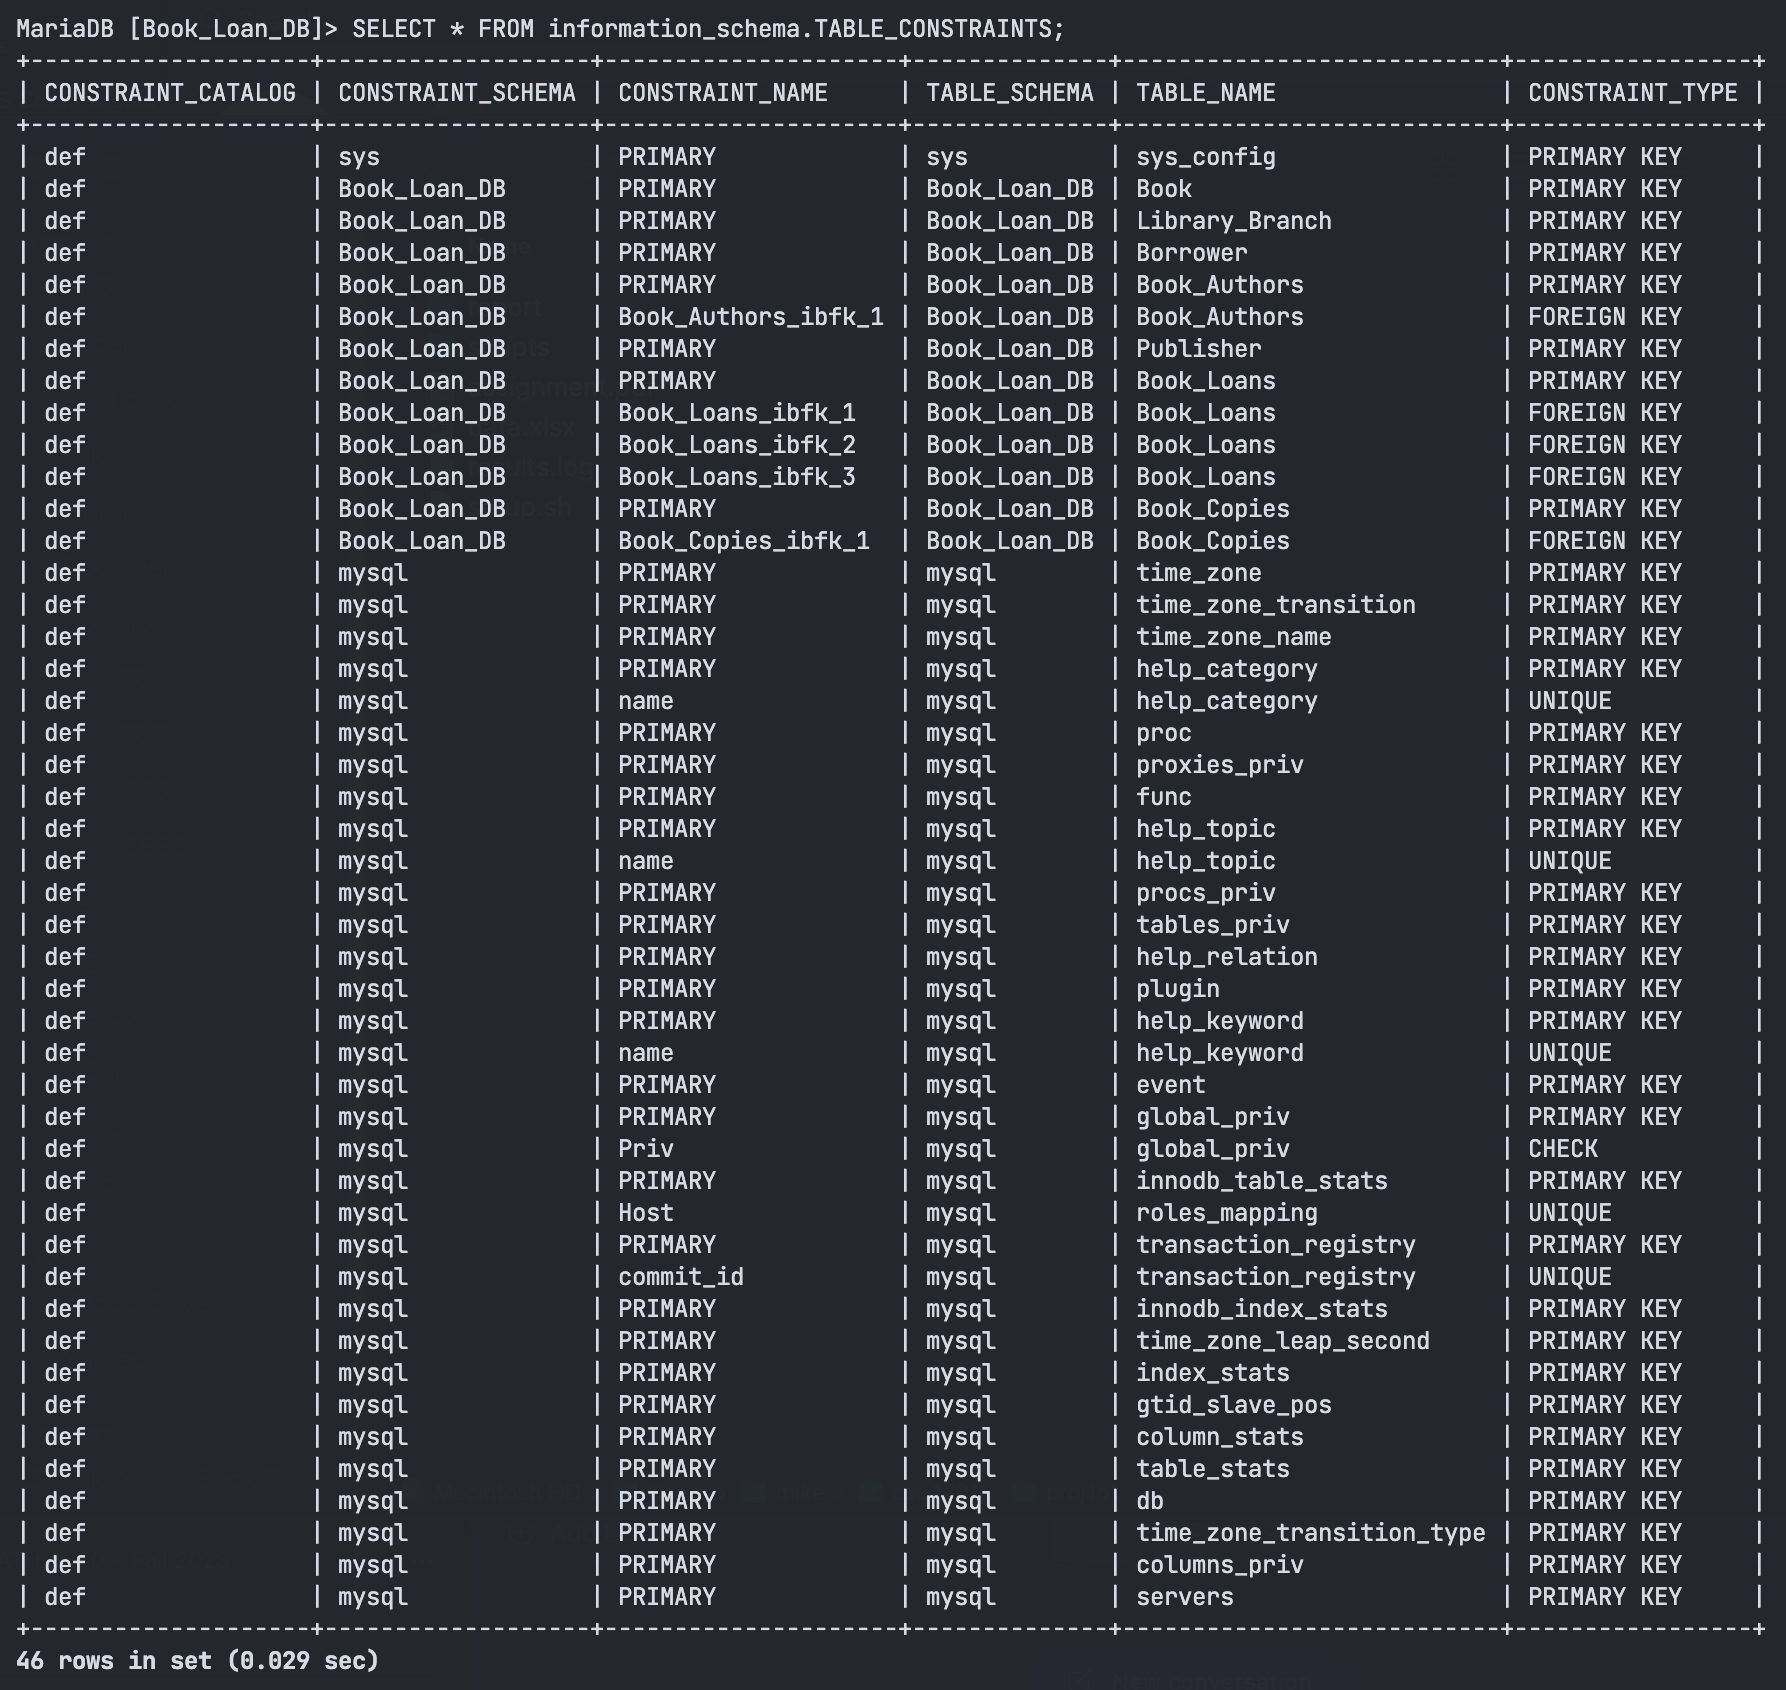
\includegraphics[width=0.8\textwidth]{images/system-table-constraints.png}
\end{center}

\newpage
\section{Verifying Table Schemas}

Below, you can see the individual table schemas from the database. In them, you can see which columns are primary keys, which columns are foreign keys, and each column's datatype.

\begin{figure}[h!]
    \begin{minipage}[b]{0.5\linewidth}
        \centering
        \caption{Book Schema}
        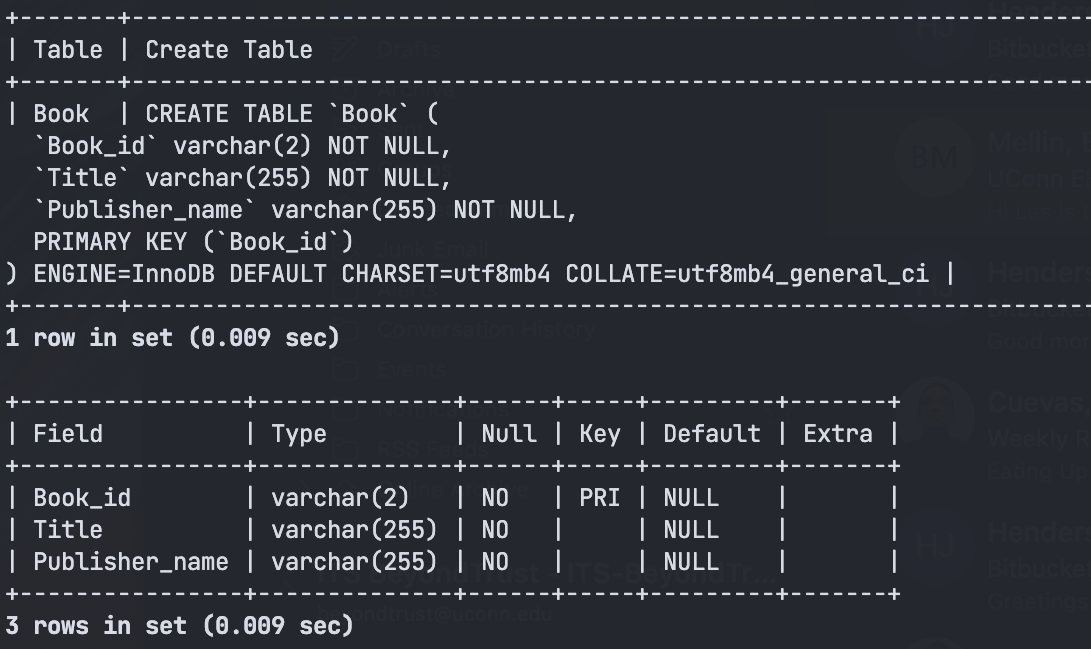
\includegraphics[width=0.8\textwidth]{images/schema-table-book.png}
        \label{fig:schema-book}
    \end{minipage}
    \hspace{0.5cm}
    \begin{minipage}[b]{0.5\linewidth}
        \centering
        \caption{Book\_Authors Schema}
        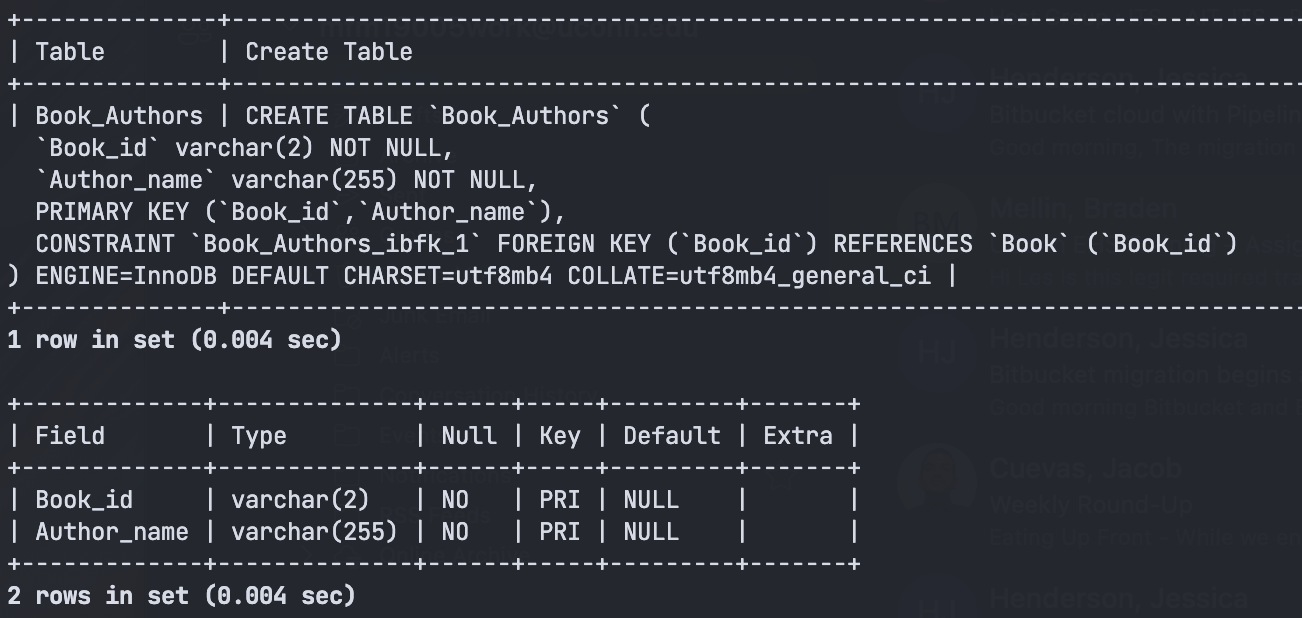
\includegraphics[width=0.8\textwidth]{images/schema-table-book-authors.png}
        \label{fig:schema-book-authors}
    \end{minipage}
\end{figure}

\begin{figure}[h!]
    \begin{minipage}[b]{0.5\linewidth}
        \centering
        \caption{Book\_Copies Schema}
        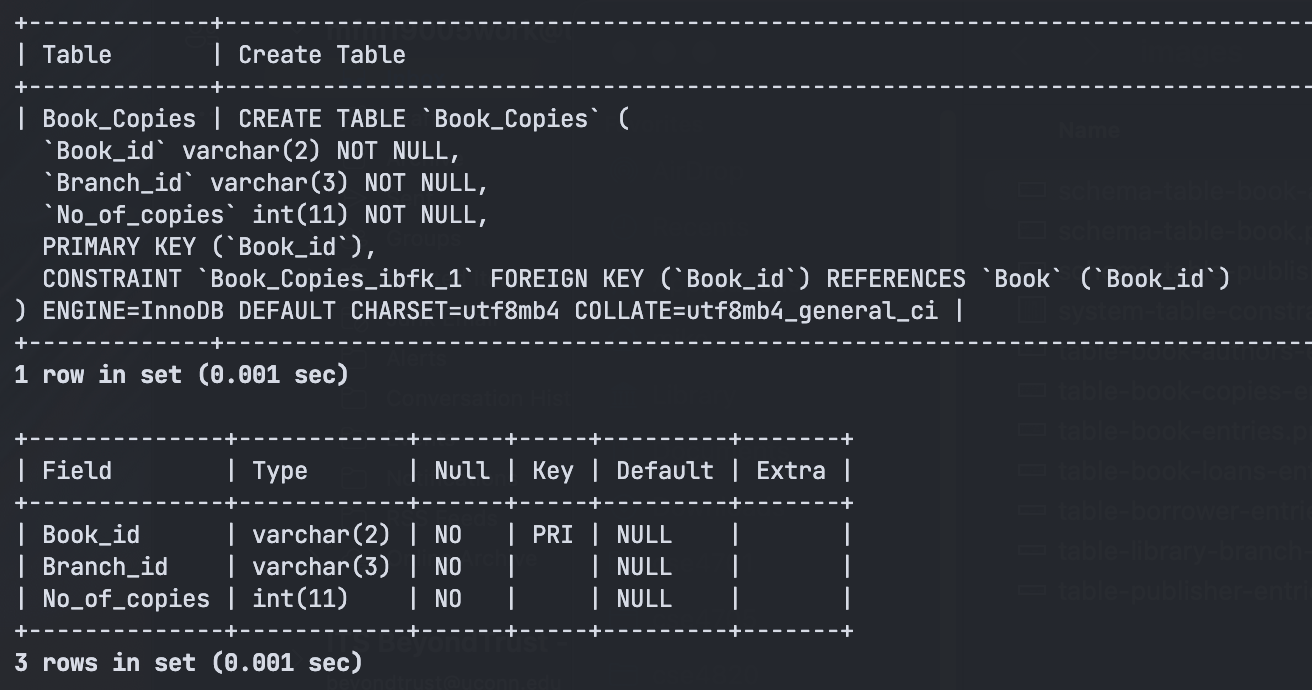
\includegraphics[width=0.8\textwidth]{images/schema-table-book-copies.png}
        \label{fig:schema-book-copies}
    \end{minipage}
    \hspace{0.5cm}
    \begin{minipage}[b]{0.5\linewidth}
        \centering
        \caption{Book\_Loans Schema}
        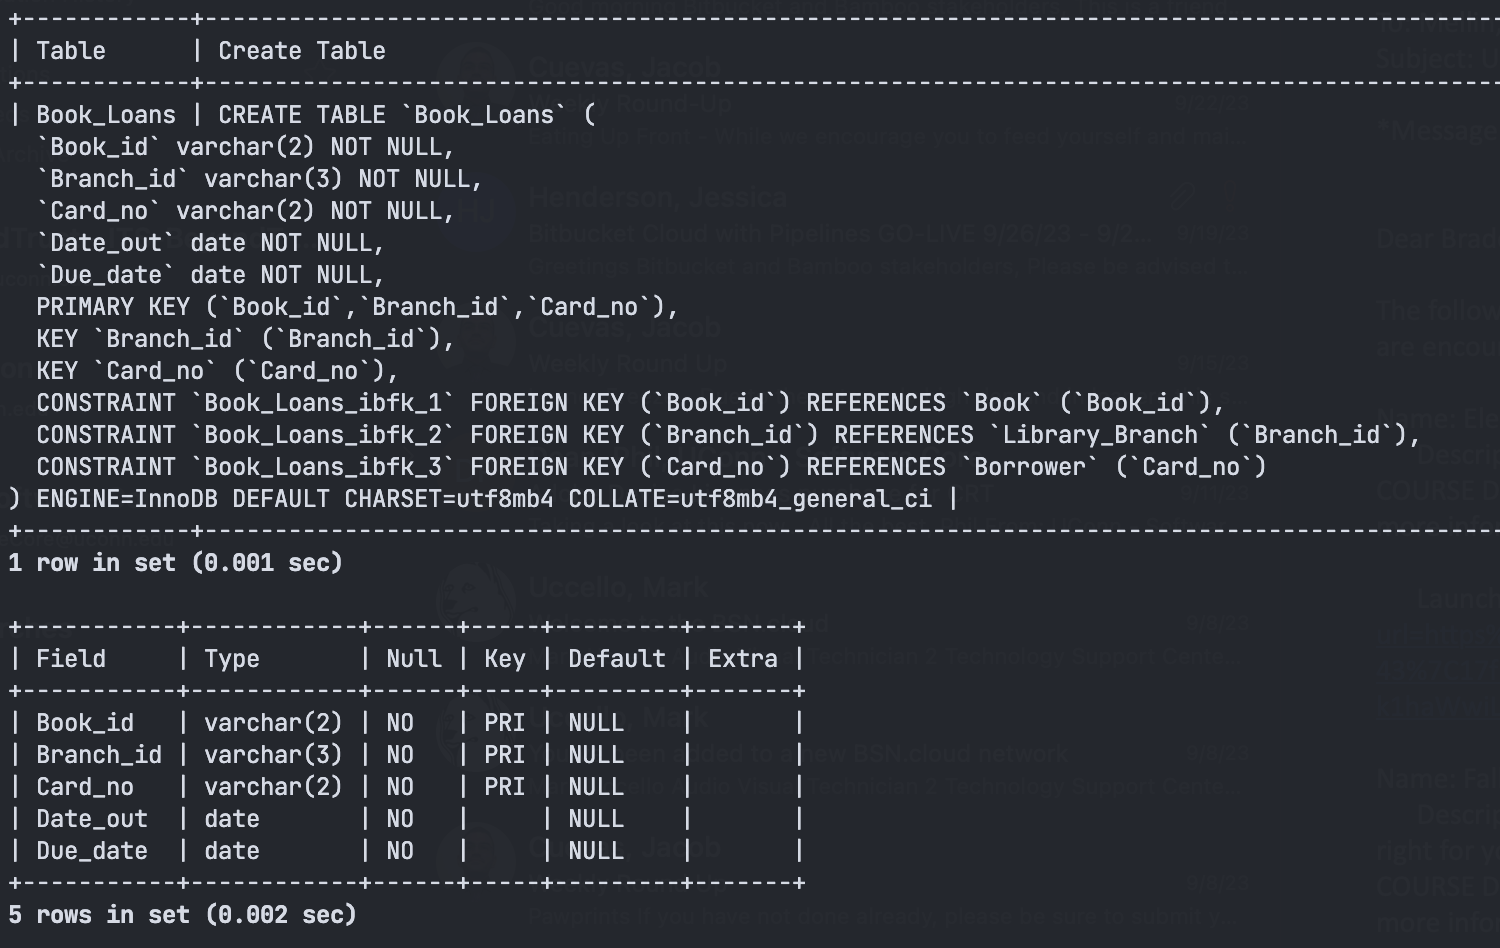
\includegraphics[width=0.8\textwidth]{images/schema-table-book-loans.png}
        \label{fig:schema-book-loans}
    \end{minipage}
    
\end{figure}

\newpage
\begin{figure}[h!]
    \begin{minipage}[b]{0.5\linewidth}
        \centering
        \caption{Borrower Schema}
        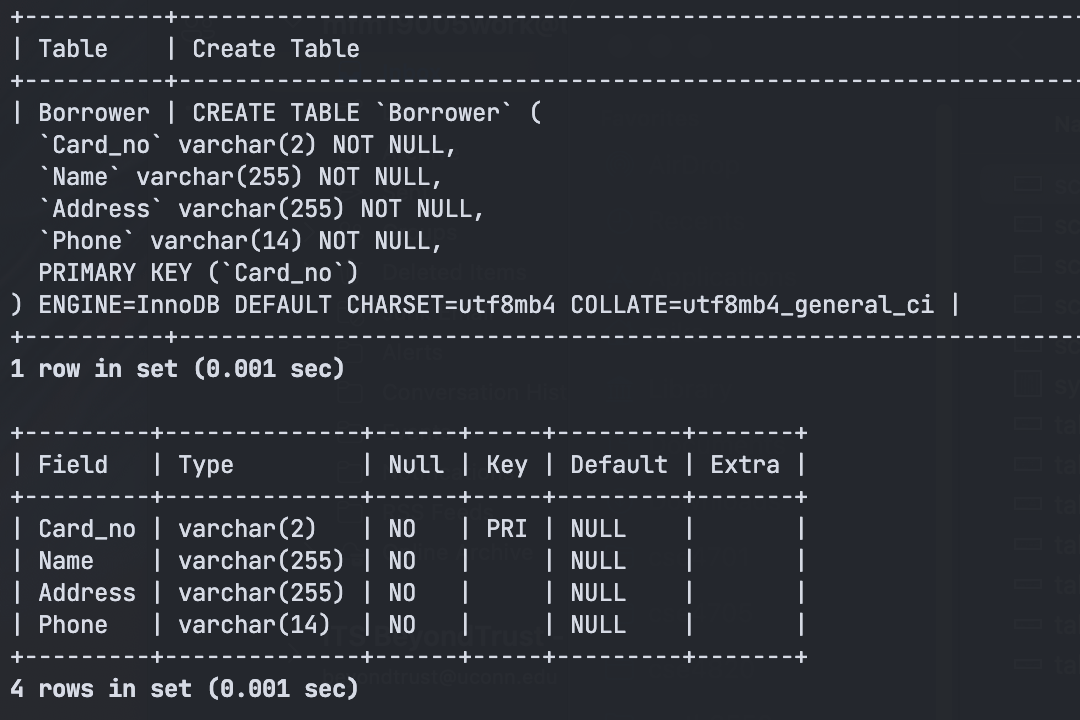
\includegraphics[width=0.8\textwidth]{images/schema-table-borrower.png}
        \label{fig:schema-borrower}
    \end{minipage}
    \hspace{0.5cm}
    \begin{minipage}[b]{0.5\linewidth}
        \centering
        \caption{Library\_Branch Schema}
        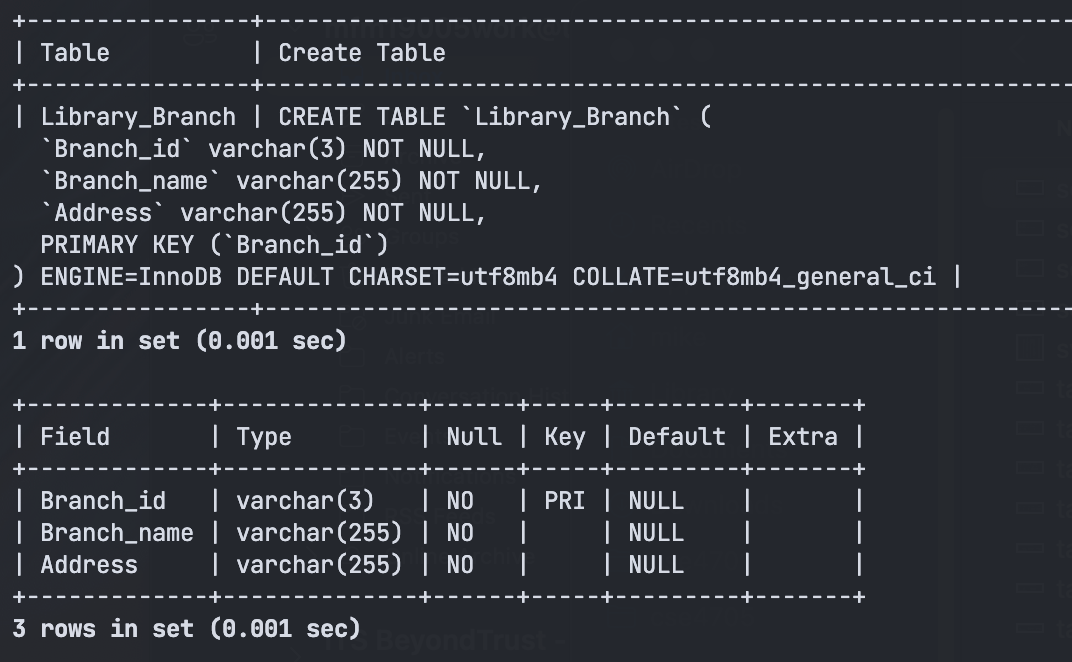
\includegraphics[width=0.8\textwidth]{images/schema-table-library-branch.png}
        \label{fig:schema-library-branch}
    \end{minipage}
\end{figure}

\begin{figure}[h!]
    \centering
    \caption{Publisher Schema}
    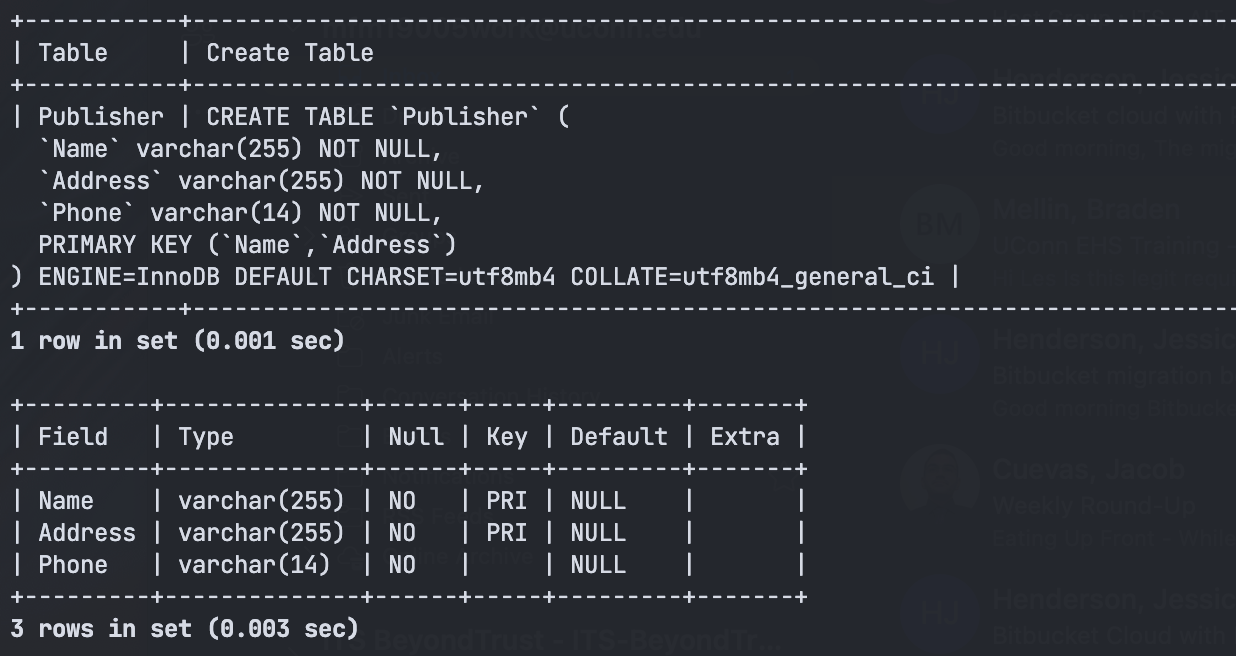
\includegraphics[width=0.5\textwidth]{images/schema-table-publisher.png}
    \label{fig:schema-publisher}
\end{figure}

\newpage
\section{Verifying Database Contents}

% minipage two columns show all images starting with "table-" in images/
\begin{figure}[h!]
    \begin{minipage}[b]{0.5\linewidth}
        \centering
        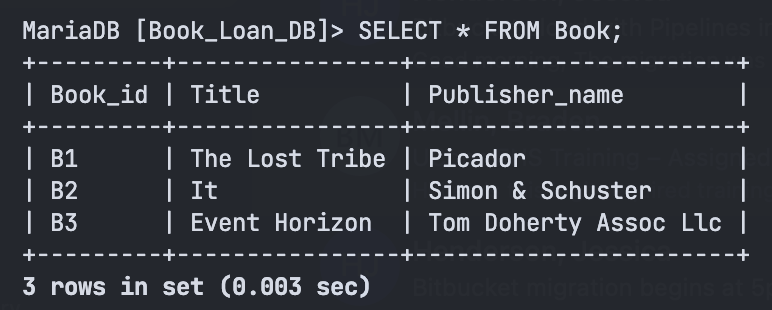
\includegraphics[width=0.8\textwidth]{images/table-book-entries.png}
        \caption{Book Values}
        \label{fig:table-book}
    \end{minipage}
    \hspace{0.5cm}
    \begin{minipage}[b]{0.5\linewidth}
        \centering
        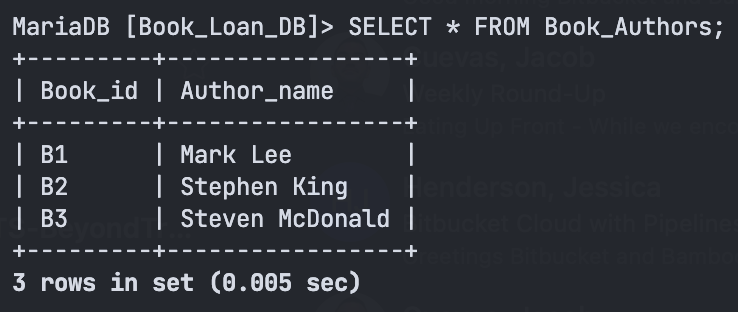
\includegraphics[width=0.8\textwidth]{images/table-book-authors-entries.png}
        \caption{Book\_Authors Values}
        \label{fig:table-book-authors}
    \end{minipage}
\end{figure}

\begin{figure}[h!]
    \begin{minipage}[b]{0.5\linewidth}
        \centering
        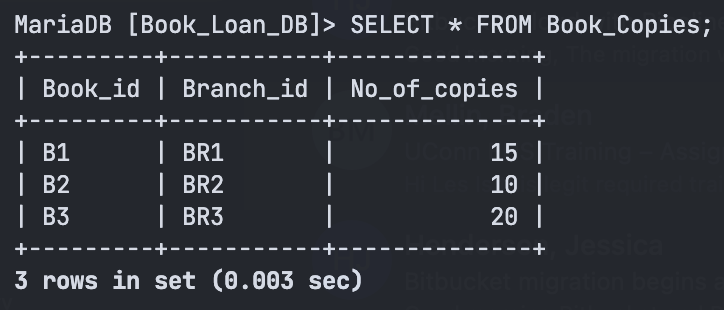
\includegraphics[width=0.8\textwidth]{images/table-book-copies-entries.png}
        \caption{Book\_Copies Values}
        \label{fig:table-book-copies}
    \end{minipage}
    \hspace{0.5cm}
    \begin{minipage}[b]{0.5\linewidth}
        \centering
        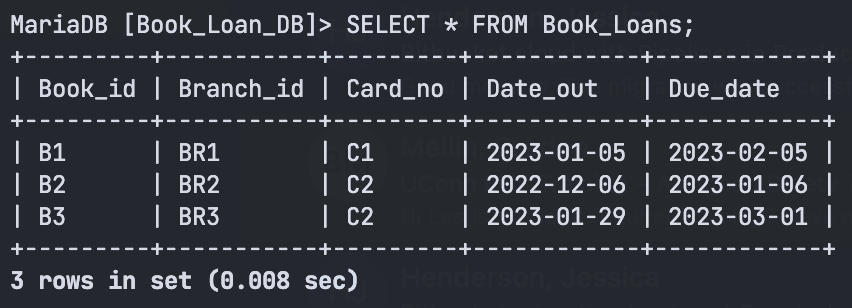
\includegraphics[width=0.8\textwidth]{images/table-book-loans-entries.png}
        \caption{Book\_Loans Values}
        \label{fig:table-book-loans}
    \end{minipage}
    
\end{figure}

\begin{figure}[h!]
    \begin{minipage}[b]{0.5\linewidth}
        \centering
        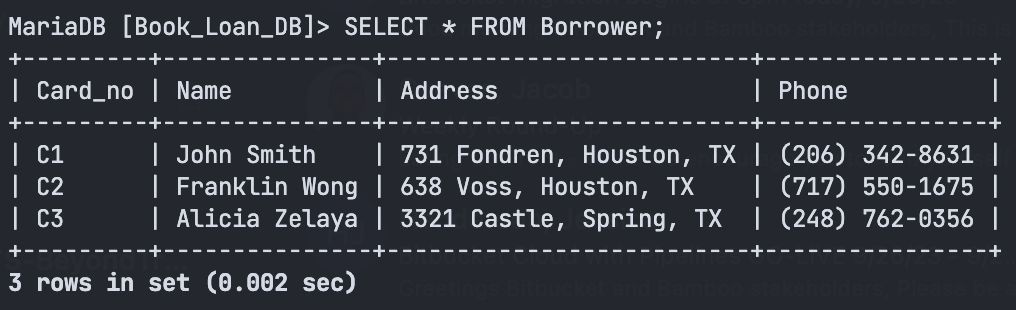
\includegraphics[width=0.8\textwidth]{images/table-borrower-entries.png}
        \caption{Borrower Values}
        \label{fig:table-borrower}
    \end{minipage}
    \hspace{0.5cm}
    \begin{minipage}[b]{0.5\linewidth}
        \centering
        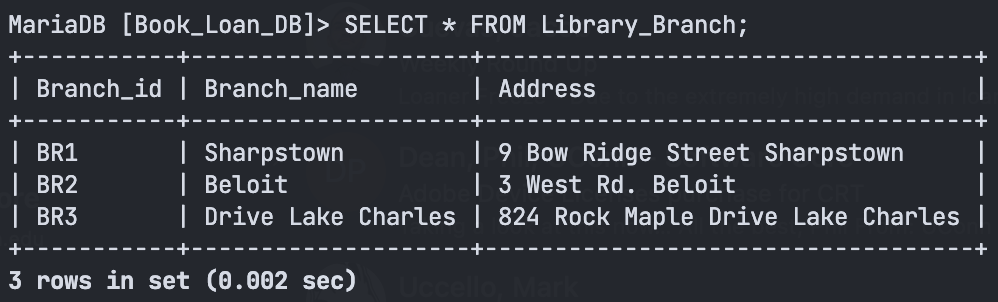
\includegraphics[width=0.8\textwidth]{images/table-library-branch-entries.png}
        \caption{Library\_Branch Values}
        \label{fig:table-library-branch}
    \end{minipage}
\end{figure}

\begin{figure}[h!]
    \centering
    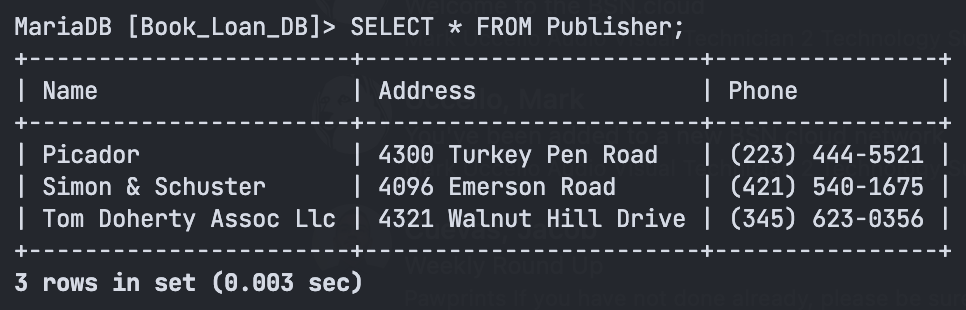
\includegraphics[width=0.5\textwidth]{images/table-publisher-entries.png}
    \caption{Publisher Values}
    \label{fig:table-publisher}
\end{figure}

\end{document}